%% LyX 2.3.4.2 created this file.  For more info, see http://www.lyx.org/.
%% Do not edit unless you really know what you are doing.
\documentclass[12pt,english]{article}
\usepackage{lmodern}
\usepackage{lmodern}
\usepackage[T1]{fontenc}
\usepackage[utf8]{inputenc}
\usepackage{geometry}
\geometry{verbose,tmargin=2.5cm,bmargin=2.5cm,lmargin=2.5cm,rmargin=2.5cm}
\usepackage{float}
\usepackage{amsmath}
\usepackage{amssymb}
\usepackage{graphicx}
\usepackage[authoryear]{natbib}

\makeatletter
\@ifundefined{date}{}{\date{}}
%%%%%%%%%%%%%%%%%%%%%%%%%%%%%% User specified LaTeX commands.

\usepackage{setspace}

%\usepackage{ae,lmodern}


%%%%%%%%%%%%%%%%%%%%%%%%%%%%%% LyX specific LaTeX commands.
%% Strike out display math with tikz
%\usepackage{tikz}
%\usetikzlibrary{calc}
%\newcommand{\lyxmathsout}[1]{%
%  \tikz[baseline=(math.base)]{
%    \node[inner sep=0pt,outer sep=0pt](math){#1};
%    \draw($(math.south west)+(2em,.5em)$)--($(math.north east)-(2em,.5em)$);
%  }
%}

%%%%%%% Billz commands %%%%%%
\usepackage{xcolor}
\newcommand{\WRY}[1]{{\color{magenta}#1}}
\newcommand{\WRYc}[1]{{\color{red}#1}}
\newcommand{\bx}{\boldsymbol{x}}
\newcommand{\bxi}{\boldsymbol{\xi} }
\usepackage[normalem]{ulem}


%%%%%%%%%%%%%%%%%%%%%%%%%%%%%% User specified LaTeX commands.
\usepackage{lineno}
\usepackage{authblk}

\DeclareMathOperator\erf{erf}



\usepackage{babel}

\makeatother

\onehalfspacing
\begin{document}
\textbf{Supporting Information} for \textit{Local intraspecific aggregation
in phytoplankton model communities: spatial scales of occurrence and
implications for coexistence}\emph{ }by C. Picoche, W.R. Young \&
F. Barraquand.

\global\long\def\thesection{S\arabic{section}}%
 \setcounter{section}{0} 
\global\long\def\thefigure{S\arabic{figure}}%
 \setcounter{figure}{0} 
\global\long\def\theequation{S\arabic{equation}}%
 \setcounter{equation}{0}

\section{Derivation of the turbulent map}

We show here how to derive a discrete-time map for turbulence from
the continuous-time formula. We consider that the velocity field $\textbf{u}^{T}=(u_{x},\,u_{y},\,u_{z})$
at position $\bx^{T}=(x,\,y,\,z)$ alternates between the three dimensions
during a period $\tau$, so that 
\begin{equation}
\textbf{u}^{T}(\bx,t)=\begin{cases}
\begin{array}{cc}
\left(U\cos(ky+\phi),0,0\right) & \text{for }n\tau\leq t<(n+\frac{1}{3})\tau\\
\left(0,U\cos(kz+\theta),0\right) & \text{for }(n+\frac{1}{3})\tau\leq t<(n+\frac{2}{3})\tau\\
\left(0,0,U\cos(kx+\psi)\right) & \text{for }(n+\frac{2}{3})\tau\leq t<(n+1)\tau.
\end{array}\end{cases}\label{eq:pierrehumber_continuous_time}
\end{equation}

The discrete-time map can be obtained by computing the displacement
over a period, between $t=n\tau$ and $t+\tau=(n+1)\tau$, with $\bx(t+\tau)=\bx(t)+\textbf{\ensuremath{\int_{n\tau}^{\left(n+1\right)\tau}}u}(\bx,t)dt$,
and knowing the initial position $\mathbf{x}(t)$. This can be solved
in three steps (eqs. \ref{eq:step1_pierrehumbert}, \ref{eq:step2_pierrehumbert}
and \ref{eq:step3_pierrehumbert}). We start with
\begin{equation}
\begin{array}{cc}
x(t+\tau/3)= & x(t)+\frac{U\tau}{3}\cos(ky(t)+\phi)\\
y(t+\tau/3)= & y(t)\\
z(t+\tau/3)= & z(t).
\end{array}\label{eq:step1_pierrehumbert}
\end{equation}
Then, 
\begin{equation}
\begin{array}{cc}
x(t+2\tau/3)= & x(t+\tau/3)\\
y(t+2\tau/3)= & y(t)+\frac{U\tau}{3}\cos(kz(t)+\theta)\\
z(t+2\tau/3)= & z(t).
\end{array}\label{eq:step2_pierrehumbert}
\end{equation}
And finally, 
\begin{equation}
\begin{array}{cc}
x(t+\tau)= & x(t+\tau/3)\\
y(t+\tau)= & y(t+2\tau/3)\\
z(t+\tau)= & z(t)+\frac{U\tau}{3}\cos(kx(t+\tau)+\psi).
\end{array}\label{eq:step3_pierrehumbert}
\end{equation}
In the third step, we need $z$ to be a function of $x(t+\tau)$,
not $x(t)$, so that the volume is conserved (the determinant of the
Jacobian matrix is equal to 1).

\section{Characteristics of standard spatial point processes}

In order to get the reader acquainted with the spatial point process
metrics that we use in the main text, we present here the analytical
formulas and corresponding figures (Fig. \ref{fig:Example-Poisson}
and \ref{fig:Example-Thomas}) for the pair correlation function,
Ripley's $K$-function and dominance index for well-known point processes.
We focus on the uniform distribution, i.e., the Poisson point process,
and a clustered distribution, the Thomas point process. The Thomas
point process is the result of a two-stage mechanism: a Poisson point
process generates ``parent points'' around which ``daughter points''
are scattered, their locations following a Gaussian distribution centered
on the parent location, with standard deviation $\sigma$. The numbers
of parents and daughters per parent follow two Poisson distributions
with mean $N_{p}$ and $N_{d}$ respectively. All solutions are given
for three-dimensional spatial distributions.

\subsection{Pair correlation function}

In the case of a Poisson point process, 
\begin{equation}
\forall r\geq0\text{, }g_{ii}(r)=1.
\end{equation}

For a Thomas point process, the expected value of the pcf is 
\begin{equation}
g_{ii}(r)=1+\frac{1}{C_{p}}\frac{1}{\left(4\pi\sigma^{2}\right)^{3/2}}e^{-\left(\frac{r^{2}}{4\sigma^{2}}\right)}
\end{equation}
where $C_{p}=N_{p}/V$ is the concentration/intensity of the parent
process in the volume $V$.\\

For a random superposition of stationary point processes with marks
(species) $i$ and $j$, $\forall i\neq j,\forall r\geq0\text{, }g_{ij}(r)=1$
\citep[ p. 326, eq. 5.3.13]{illian2008statistical}.

\subsection{Ripley's $K$-function}

In the case of a Poisson point process, 
\begin{equation}
\forall r\geq0\text{, }K_{ii}(r)=\frac{4}{3}\pi r^{3}.\label{eq:k_poisson}
\end{equation}

For a Thomas point process, 
\begin{equation}
K_{ii}(r)=\frac{4}{3}\pi r^{3}+\frac{1}{C_{p}\sigma\sqrt{\pi}}\left(\sigma\sqrt{\pi}\erf\left(\frac{r}{2\sigma}\right)-re^{-\left(\frac{r}{2\sigma}\right)^{2}}\right).\label{eq:k_thomas}
\end{equation}

For a random superposition of stationary point processes, $K_{ij}(r)=\frac{4}{3}\pi r^{3}$
\citep[p. 324, eq. 5.3.5]{illian2008statistical}.

\subsection{Dominance index}

In the Poisson point process, $K_{ii}(r)=K_{ij}(r)$, which means
that the dominance index can be reduced to ratios of concentrations:
\begin{equation}
\mathcal{D}_{i}(r)=\frac{C_{i}}{\sum_{j=1}^{S}C_{j}}.
\end{equation}

In the Thomas process, using eq. \ref{eq:k_thomas}, 
\begin{equation}
\mathcal{D}_{i}(r)=\frac{C_{i}\left(\frac{4}{3}\pi r^{3}+\frac{F(r)}{C_{p,i}}\right)}{C_{i}\frac{F(r)}{C_{p,i}}+\sum_{j}C_{j}\frac{4}{3}\pi r^{3}}
\end{equation}
with $F(r)=\frac{1}{\sigma\sqrt{\pi}}\left(\sigma\sqrt{\pi}\erf\left(\frac{r}{2\sigma}\right)-re^{-\left(\frac{r}{2\sigma}\right)^{2}}\right)$.

\begin{figure}[H]
\begin{centering}
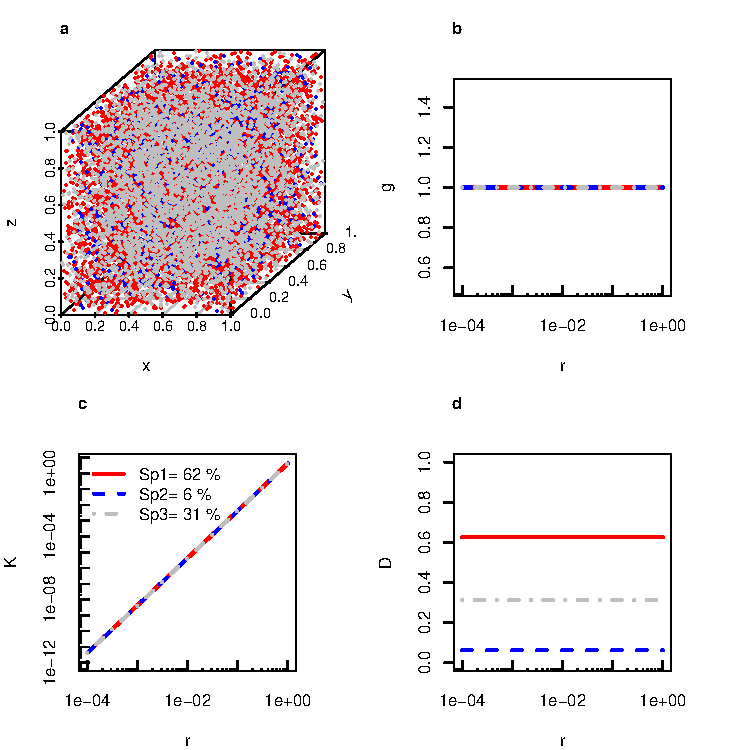
\includegraphics[width=.79\textwidth]{../code/figure/example_Poisson_distribution}
\par\end{centering}
\caption{Example of spatial distribution (a) and theoretical pair correlation
function (b), Ripley's $K$-function (c) and dominance index (d) for
a Poisson point process in 3-species communities with different intensities
(10000 cm$^{-3}$, 1000 cm$^{-3}$, 5000 cm$^{-3}$; proportions in
the community are given in the figure). \label{fig:Example-Poisson}}
\end{figure}

\begin{figure}[H]
\begin{centering}
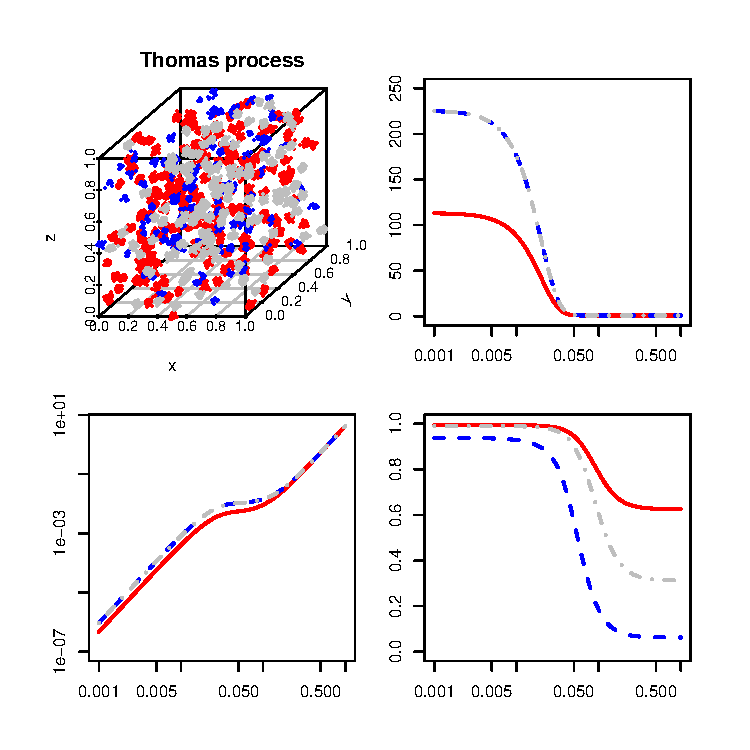
\includegraphics[width=0.79\textwidth]{../code/figure/example_Thomas_distribution}
\par\end{centering}
\caption{Example of spatial distribution (a) and theoretical pair correlation
function (b), Ripley's $K$-function (c) and dominance index (d) for
a Thomas point process in 3-species communities with different parent
intensities (200 cm$^{-3}$, 100 cm$^{-3}$, 100 cm$^{-3}$), and
different children per parent intensities (50, 10, 50; final proportions
in the communities are given in the figure), with $\sigma=0.01$.\label{fig:Example-Thomas}}
\end{figure}


\section{Convergence in time of the spatial characteristics of the BBM}

The theoretical formulas of $g$, $K$ and $\mathcal{D}$ can be used
to study the behaviour of the BBM. In the absence of advection, convergence
cannot be reached in a reasonable timeframe: even a week is not long
enough for the steady-state solution to be reached (see blue line
in Fig. \ref{fig:Theoretical-convergence}). However, the population-at-equilibrium
hypothesis that we use cannot hold for such a long amount of time,
which led us to use the time-dependent formulas shown in Eqs. 5, 9
and 12 in the main text.

\begin{figure}[H]
\begin{centering}
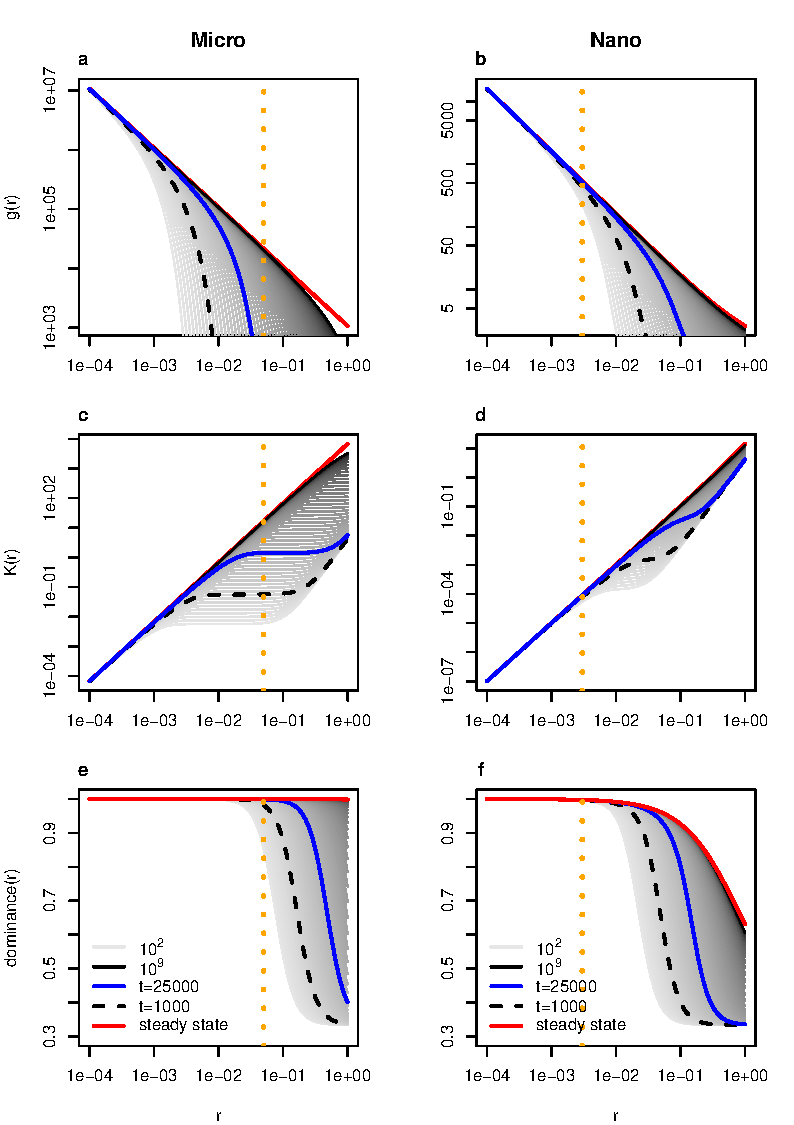
\includegraphics[height=0.82\textheight]{../code/figure/convergence_wo_advection} 
\par\end{centering}
\caption{Intraspecific pair correlation function (a, b), Ripley's $K$-function
(c,d) and dominance index (e,f) as a function of distance (in cm)
for microphytoplankton and nanophytoplankton in the absence of advection,
for a single species in a 3-species community with an even abundance
distribution. Shorter timeframes are shown with light grey lines while
longer ones are shown with darker shades. The theoretical value at
steady state is shown in red. The duration currently used in the simulations
($t=1000\tau$) is shown with dashed black lines. A duration corresponding
to a week is shown with solid blue lines. Dotted orange lines correspond
to the distance threshold for interaction.\label{fig:Theoretical-convergence}}
\end{figure}

In a similar fashion, we can show with the dominance index (Fig. \ref{fig:Theoretical-dom})
the progressive clustering of individuals with time when advection
is absent, and compare it to the steady state this time \emph{with}
advection. We see that even after a short period of time ($t=100\tau$),
the dominance index without advection is larger than with advection,
and this spatial aggregation only grows with time in absence of turbulent
advection.

\begin{figure}[H]
\begin{centering}
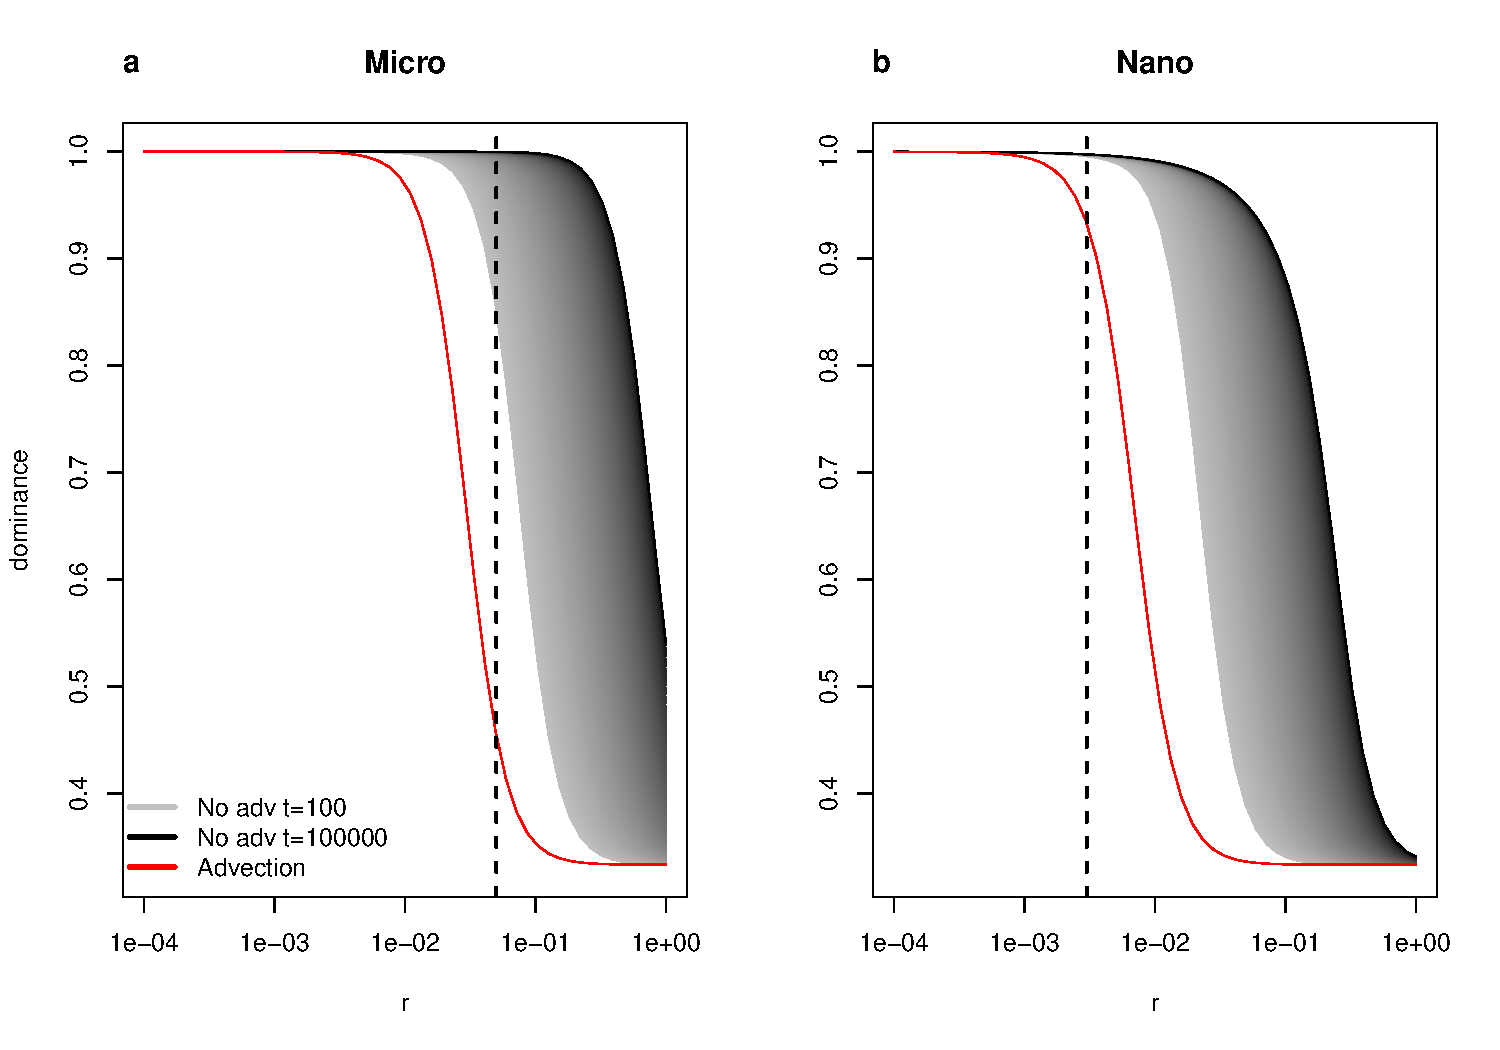
\includegraphics[width=0.8\textwidth]{../code/figure/theory_dominance} 
\par\end{centering}
\caption{Theoretical dominance indices as a function of the distance (in cm)
from a particle of a given species, for a microphytoplankton (a) and
nanophytoplankton (b) 3-species community with an even abundance distribution,
with (red line) and without (grey to black lines, with darker lines
for longer simulations) advection. The vertical dashed line corresponds
to the distance threshold for interaction. \label{fig:Theoretical-dom}}
\end{figure}


\section{Computation of the pair correlation function and Ripley's $K$-function}

The algorithm for pcf computation was adapted from the function \verb|pcf3est|
in spatstat 2.2-0 \citep{baddeley_spatstat} and slightly modified
to compute the interspecific pcf (i.e., the pcf for marked point processes).

The pcf estimate $\hat{g}_{ij}(r)$ is computed via the use of the
Epanechnikov kernel $\kappa_{E}$ with bandwidth $\delta$, i.e. 
\begin{equation}
\begin{array}{ccc}
\hat{g}_{ij}(r) & = & \frac{1}{\hat{C_{i}}}\frac{1}{\hat{C_{j}}}\frac{1}{4\pi r^{2}}\sum_{k\in i}\sum_{l\in j}\kappa_{E}(r-||\bx_{k}-\bx_{l}||)w(\bx_{k},\bx_{l})\end{array}\label{eq:pcf_estimate}
\end{equation}
where $w(\bx_{k},\bx_{l})$ is the Ohser translation correction estimator
\citep{ohser_estimators_1983} and the kernel is defined as follow.
\begin{equation}
\kappa_{E}(x)=\begin{cases}
\frac{3}{4\delta}\left(1-\frac{x^{2}}{\delta^{2}}\right) & \text{for }-\delta\leq x\leq\delta\\
0 & \text{otherwise}.
\end{cases}
\end{equation}

The estimate $\hat{g}_{ij}(r)$ is therefore very sensitive to the
bandwidth: if it is too small, the estimate is noisy and may even
be missing several pairs of points; if it is too large, the smoothing
might be so important that values are strongly underestimated. In
spatstat 2.2-0 \citep{baddeley_spatstat}, the bandwidth default value
is $\delta=0.26C^{-1/3}$. The pcf computation function was first
tested on standard distributions (with the default bandwidth), then
on the Brownian Bug Model (with different bandwidths, see Fig. \ref{fig:bandwidth_BBM}).

Estimates of the Ripley's $K$-function were also computed with the
Ohser translation correction estimator but did not require any kernel
smoothing. The same computation could be done using wrapped-around
boundary conditions (for pcf estimation; for simulation we always
consider periodic boundary conditions).

\subsection{Standard point processes}

\begin{figure}[H]
\begin{centering}
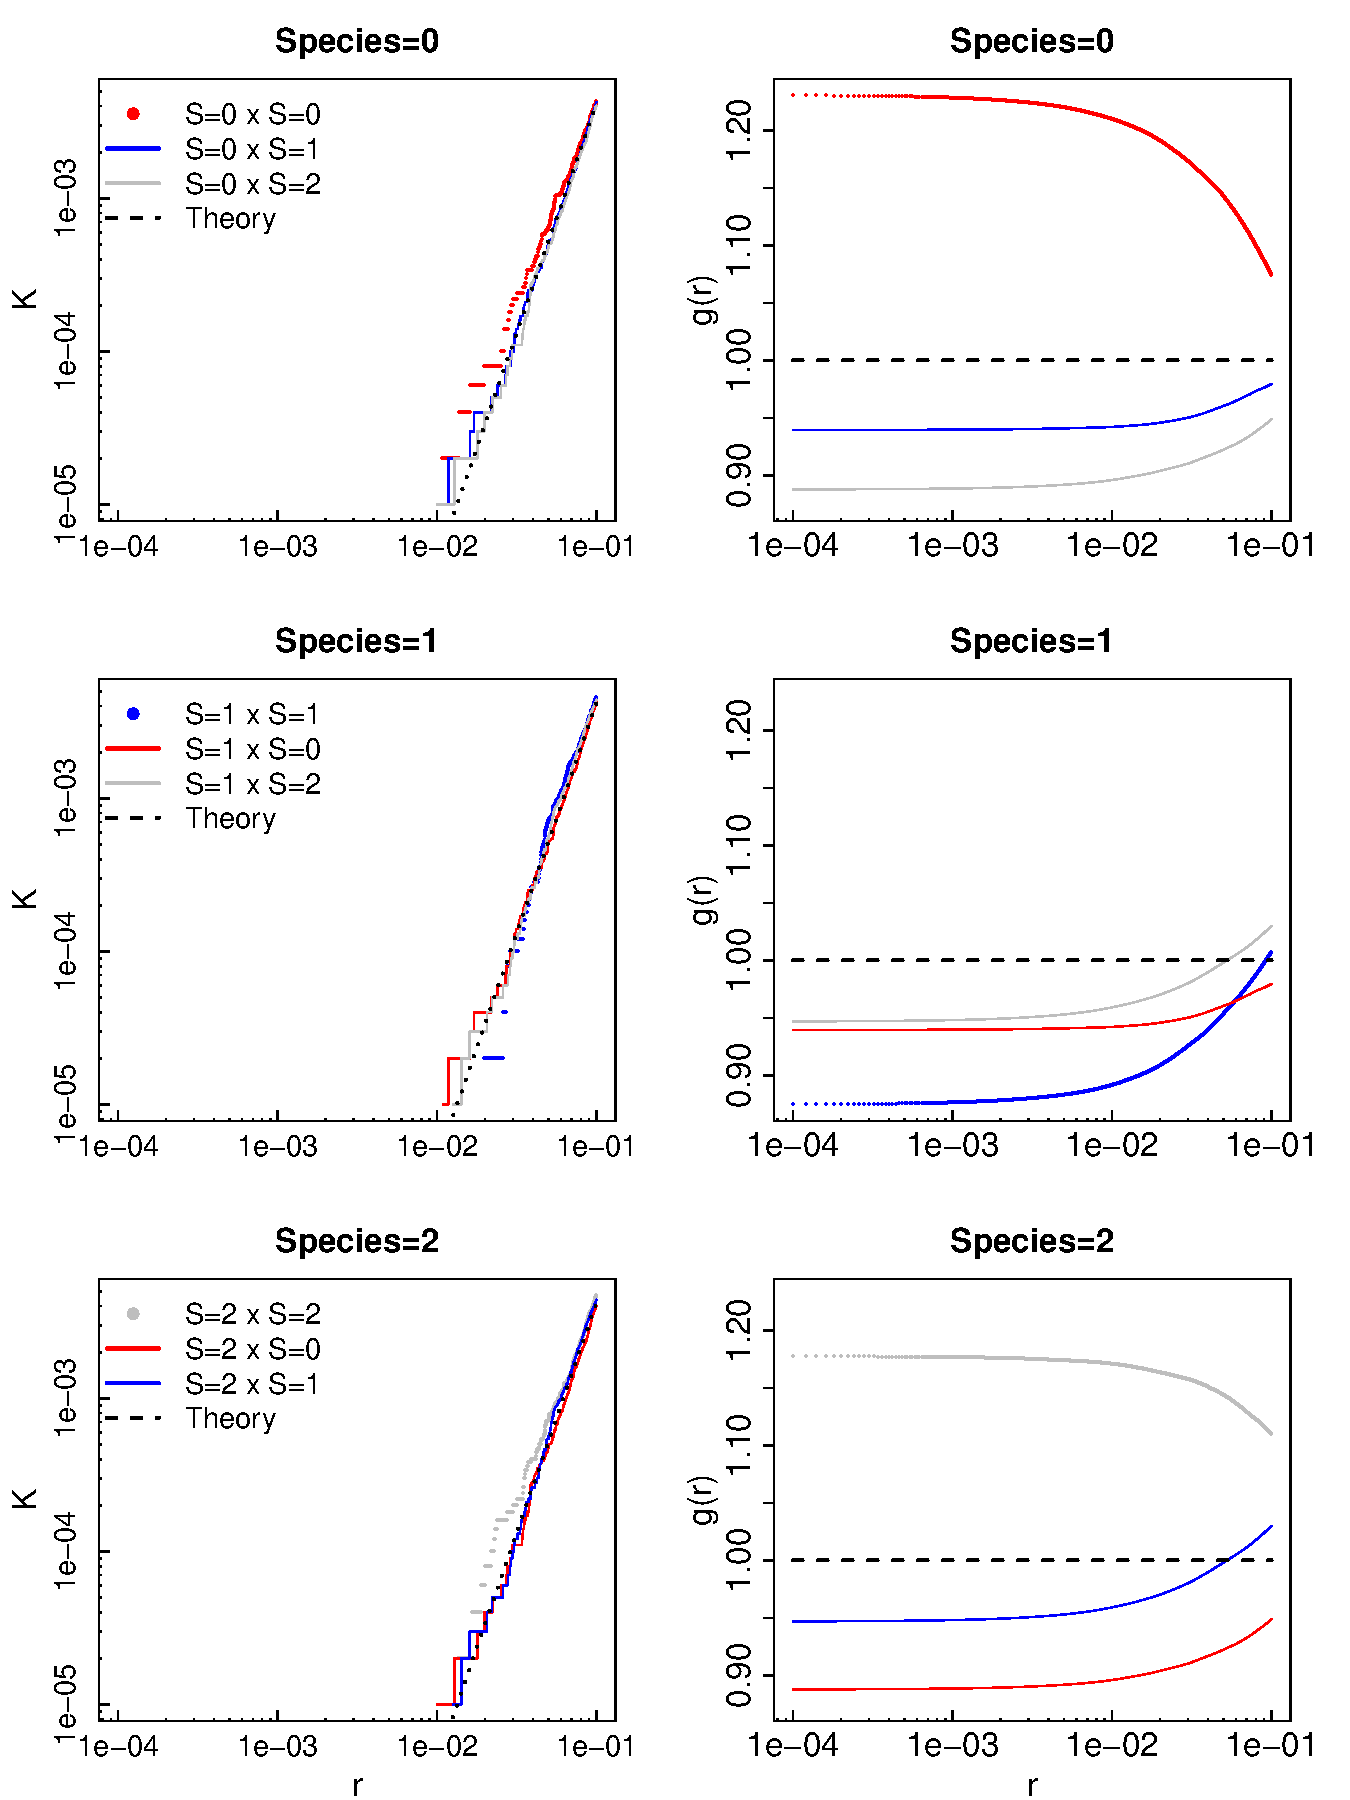
\includegraphics[height=0.8\textheight]{../code/figure/K_PCF_Poisson} 
\par\end{centering}
\caption{Intra- and inter-specific Ripley's $K$-function and pair correlation
function values as a function of distance (in cm) for 3 species following
a Poisson process with intensity 10 cm$^{-3}$, in a volume of 1000
cm$^{3}$. Values computed from our simulations (circles and solid
lines for intra- and interspecific values, respectively) are compared
with theoretical formulas (dotted lines). Note that theoretical values
are the same for intra and interspecific indices for the Poisson distribution.
Colors correspond to the different species (red for species 0, blue
for species 1, grey for species 2).}
\end{figure}

\begin{figure}[H]
\begin{centering}
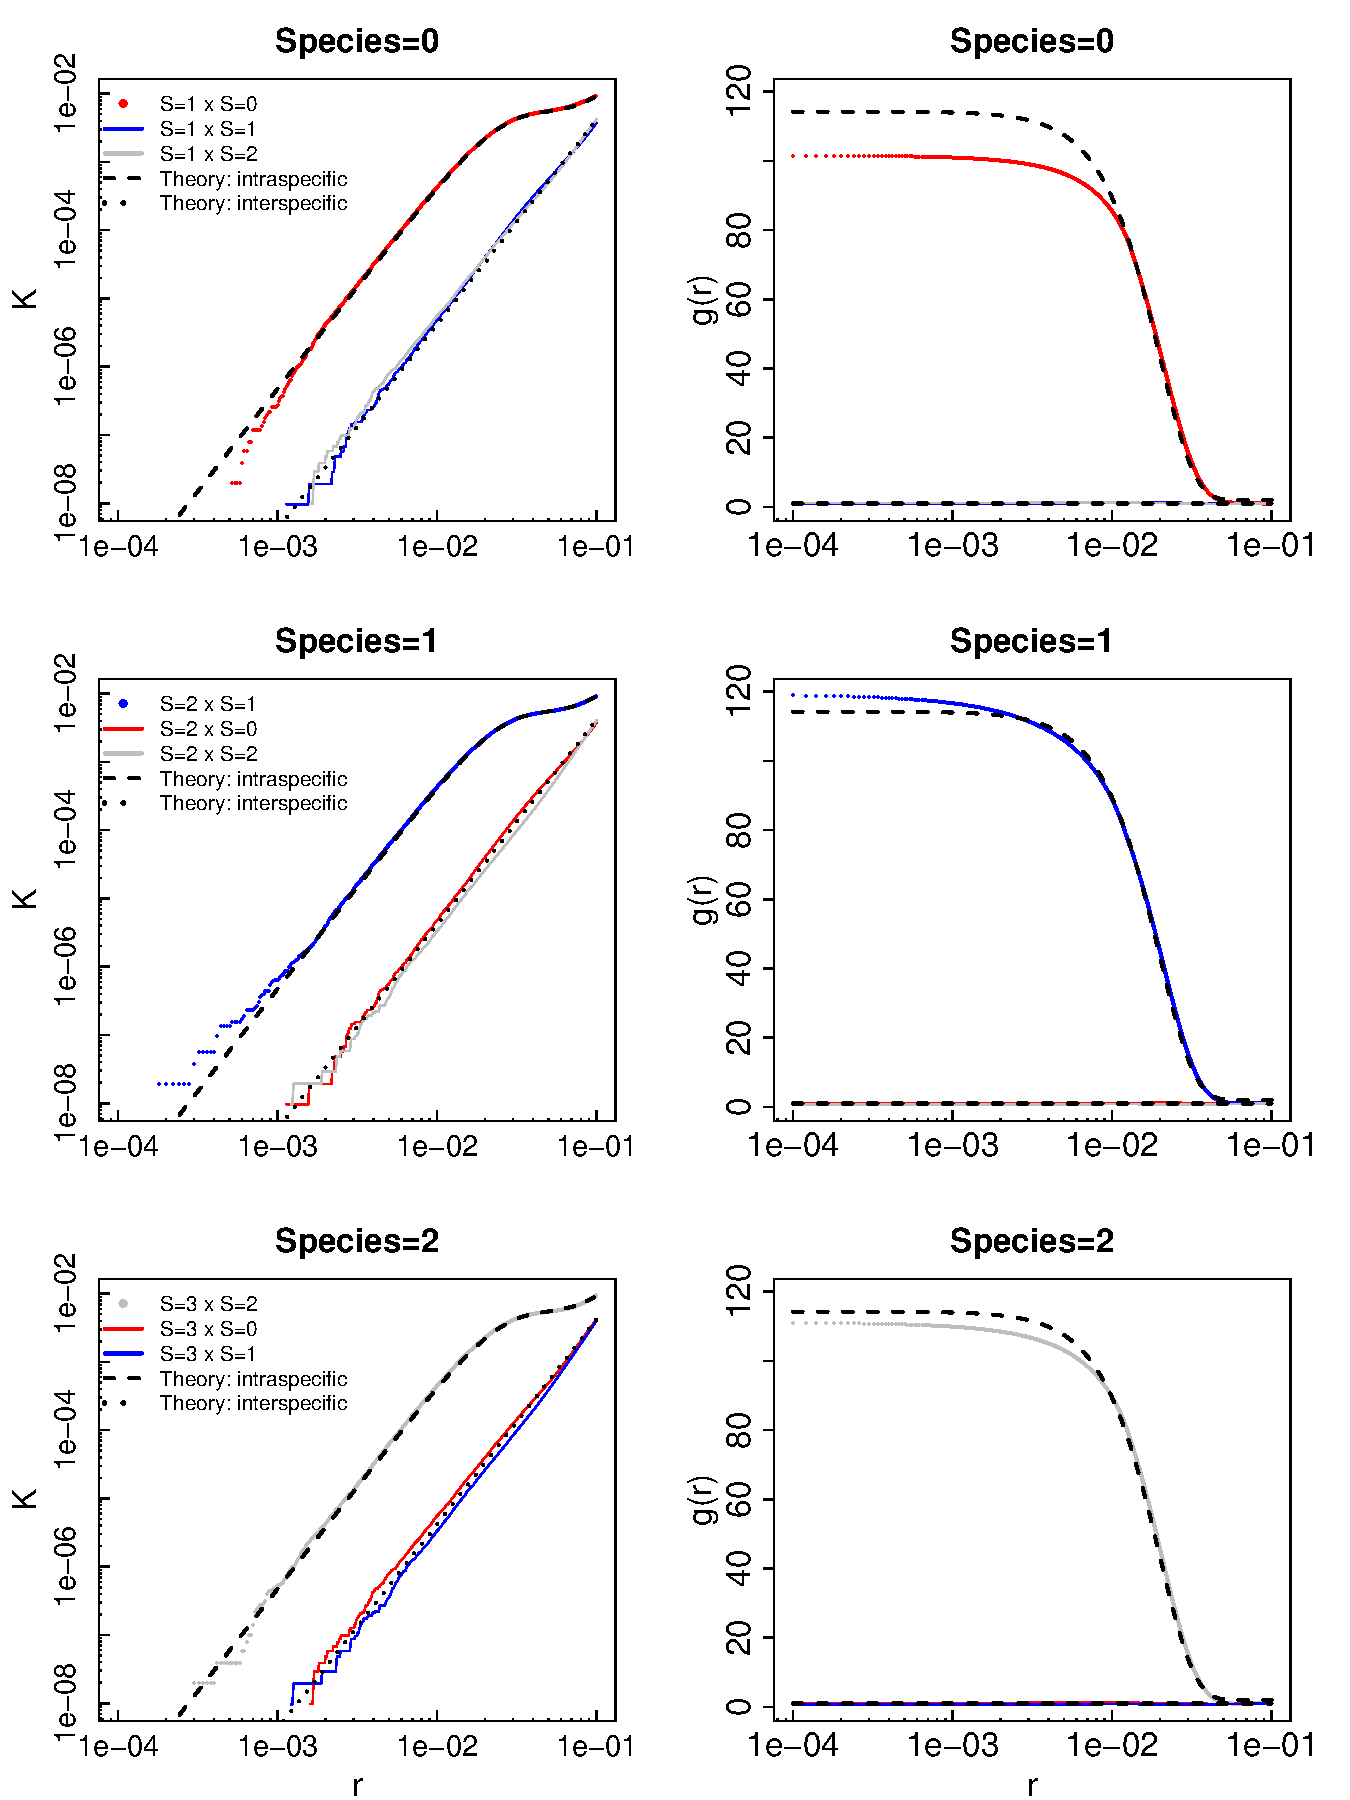
\includegraphics[height=0.8\textheight]{../code/figure/K_PCF_Thomas} 
\par\end{centering}
\caption{Intra- and inter-specific Ripley's $K$-function and pair correlation
function values as a function of distance (in cm) for 3 species following
a Thomas process with parent intensity $C_{p}=200$ cm$^{-3}$, number
of children per parent $N_{c}=50$, in a volume of 1 cm$^{3}$, $\sigma=0.01$
and $\delta\approx0.01$2. Values computed from our simulations (circles
and solid lines for intra- and interspecific values, respectively)
are compared with theoretical formulas (dashed and dotted lines for
intra- and interspecific values, respectively). Colors correspond
to the different species (red for species 0, blue for species 1, grey
for species 2). }
\end{figure}


\subsection{Brownian Bug Model}

While the pcf was one of the first indices that we intended to use,
we quickly realized that the combination of the large range of distances
we wanted to explore (from $10^{-4}$ to 1 cm) and the low density
of individuals, at least for microphytoplankton, made the estimation
difficult as the choice of the bandwidth was critical. We give an
example of the sensitivity of the pcf computation to the bandwidth
below (Fig. \ref{fig:bandwidth_BBM}).

\begin{figure}[H]
\begin{centering}
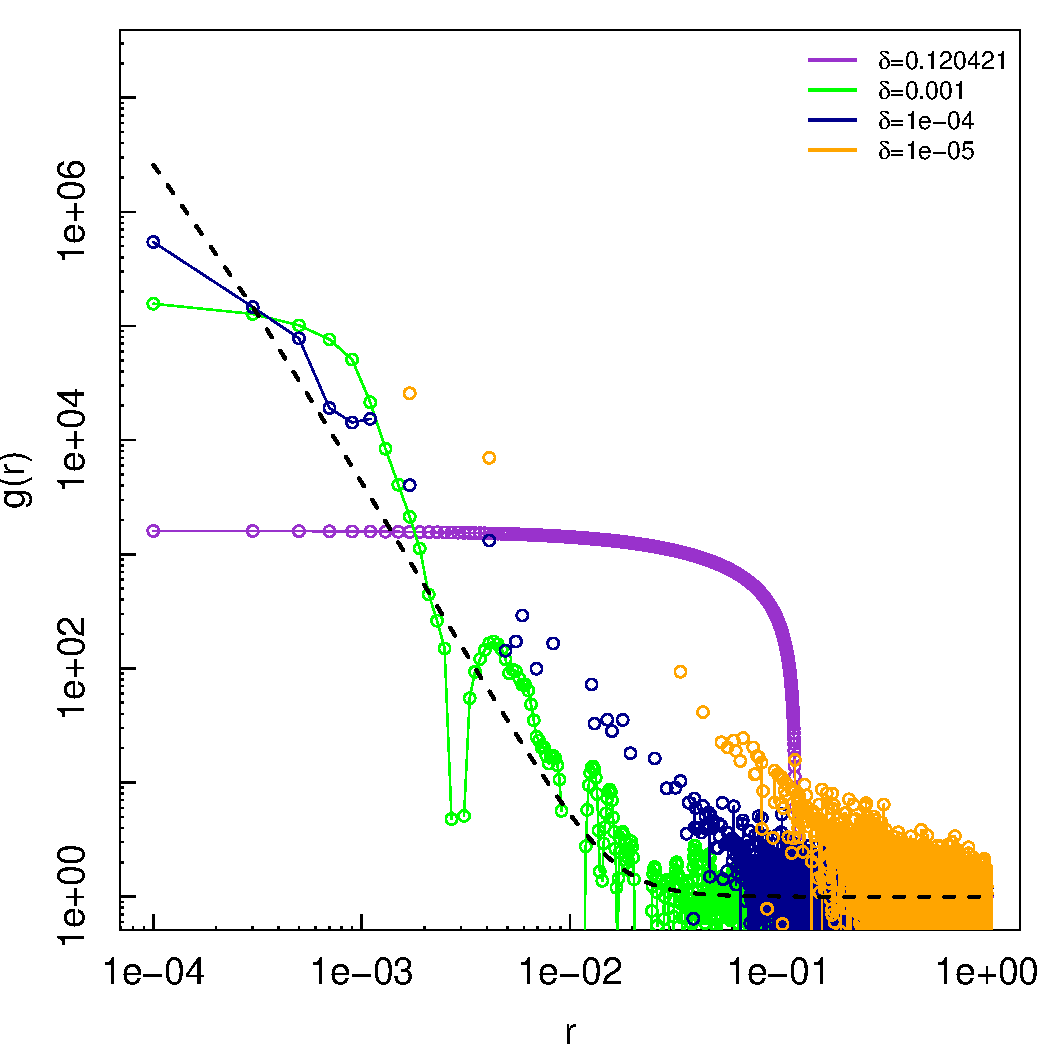
\includegraphics[width=0.6\textwidth]{../code/figure/bandwidth_BBM} 
\par\end{centering}
\caption{Intraspecific pair correlation function as a function of distance
(in cm) computed for the Brownian Bug Model with microphytoplankton
individuals, after 1000 time steps, with different values of the bandwidth
$\delta$. The dashed line indicates the theoretical pcf.\label{fig:bandwidth_BBM} }
\end{figure}

We decided, realizing that it would be very challenging to obtain
a non-noisy pcf curve matching the theoretical expectation, to focus
on Ripley's $K$-function whose cumulative nature helps the estimation
process, which enabled us to compute the dominance index without having
to calibrate a bandwidth beforehand.

\section{Spatial distributions}

\begin{figure}[H]
\begin{centering}
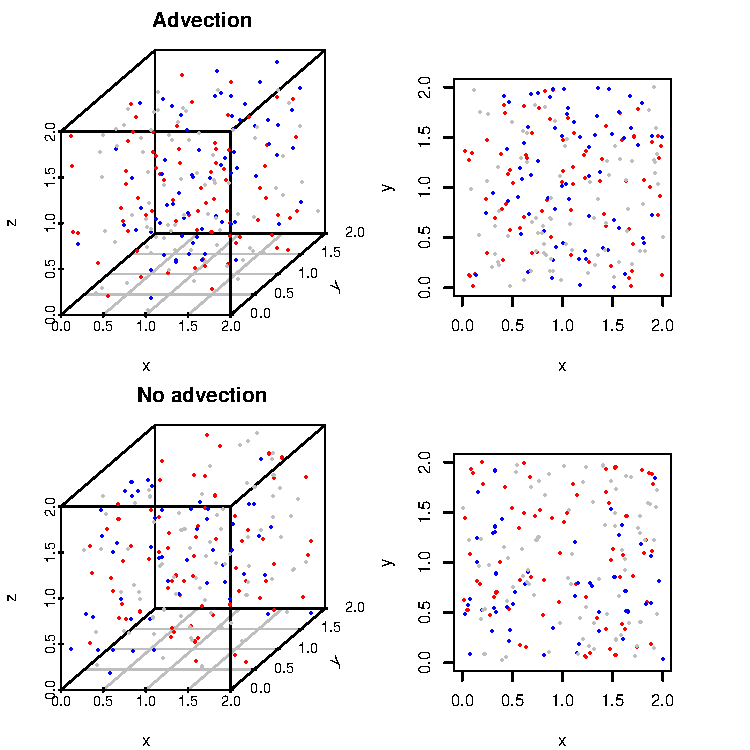
\includegraphics[width=0.99\textwidth]{../code/figure/spatial_distribution_zoom_micro0} 
\par\end{centering}
\caption{Spatial distributions of a 3-species community of microphytoplankton
with and without advection with density $C=10$ cells~cm$^{-3}$
after 1000 time steps. Each color corresponds to a different species.
On the left-hand side, only a zoom on a $2\times2\times2$ cm$^{3}$
cube is shown, and its projection on the x-y plane is shown on the
right-hand side. \label{fig:Spatial-distributions}}
\end{figure}

\section{Sensitivity to the computation of the advection parameter}

To compute the value of the maximum velocity of an organism in our
model at the Kolmogorov scale, we used the formula $\text{Re}=U/k\nu\approx1$
where $k$ is the smallest wavenumber associated with turbulence.
However, we could compute the Reynolds number with another, slightly
different formula, using the equivalent sphere diameter ($L_{v}$)
of our system (eq. \ref{eq:re_lv}). In this case, $\text{Re}=UL_{v}/\nu$
and 
\begin{equation}
\begin{array}{cccc}
 & \frac{4}{3}\pi\left(\frac{L_{v}}{2}\right)^{3} & = & L_{c}^{3}\\
\Leftrightarrow & L_{v} & = & 2L_{c}\left(\frac{3}{4\pi}\right)^{1/3}\\
\Leftrightarrow & L_{v} & = & 1.24\text{ cm}.
\end{array}\label{eq:re_lv}
\end{equation}
If we use $U\approx\nu/L_{v}$, we obtain $U\approx8.1\times10^{-5}$ m~s$^{-1}$. Using $U\tau/3=0.5$ cm, we then have $\tau=185\text{ s}=2.1\times10^{-3}$ d. This value of $U$ is associated to an estimated $\gamma=164$ d$^{-1}$. As could be expected,
when the flow velocity $U$ decreases, mixing decreases (Fig. \ref{fig:Dominance_advection}).

\begin{figure}[H]
\begin{centering}
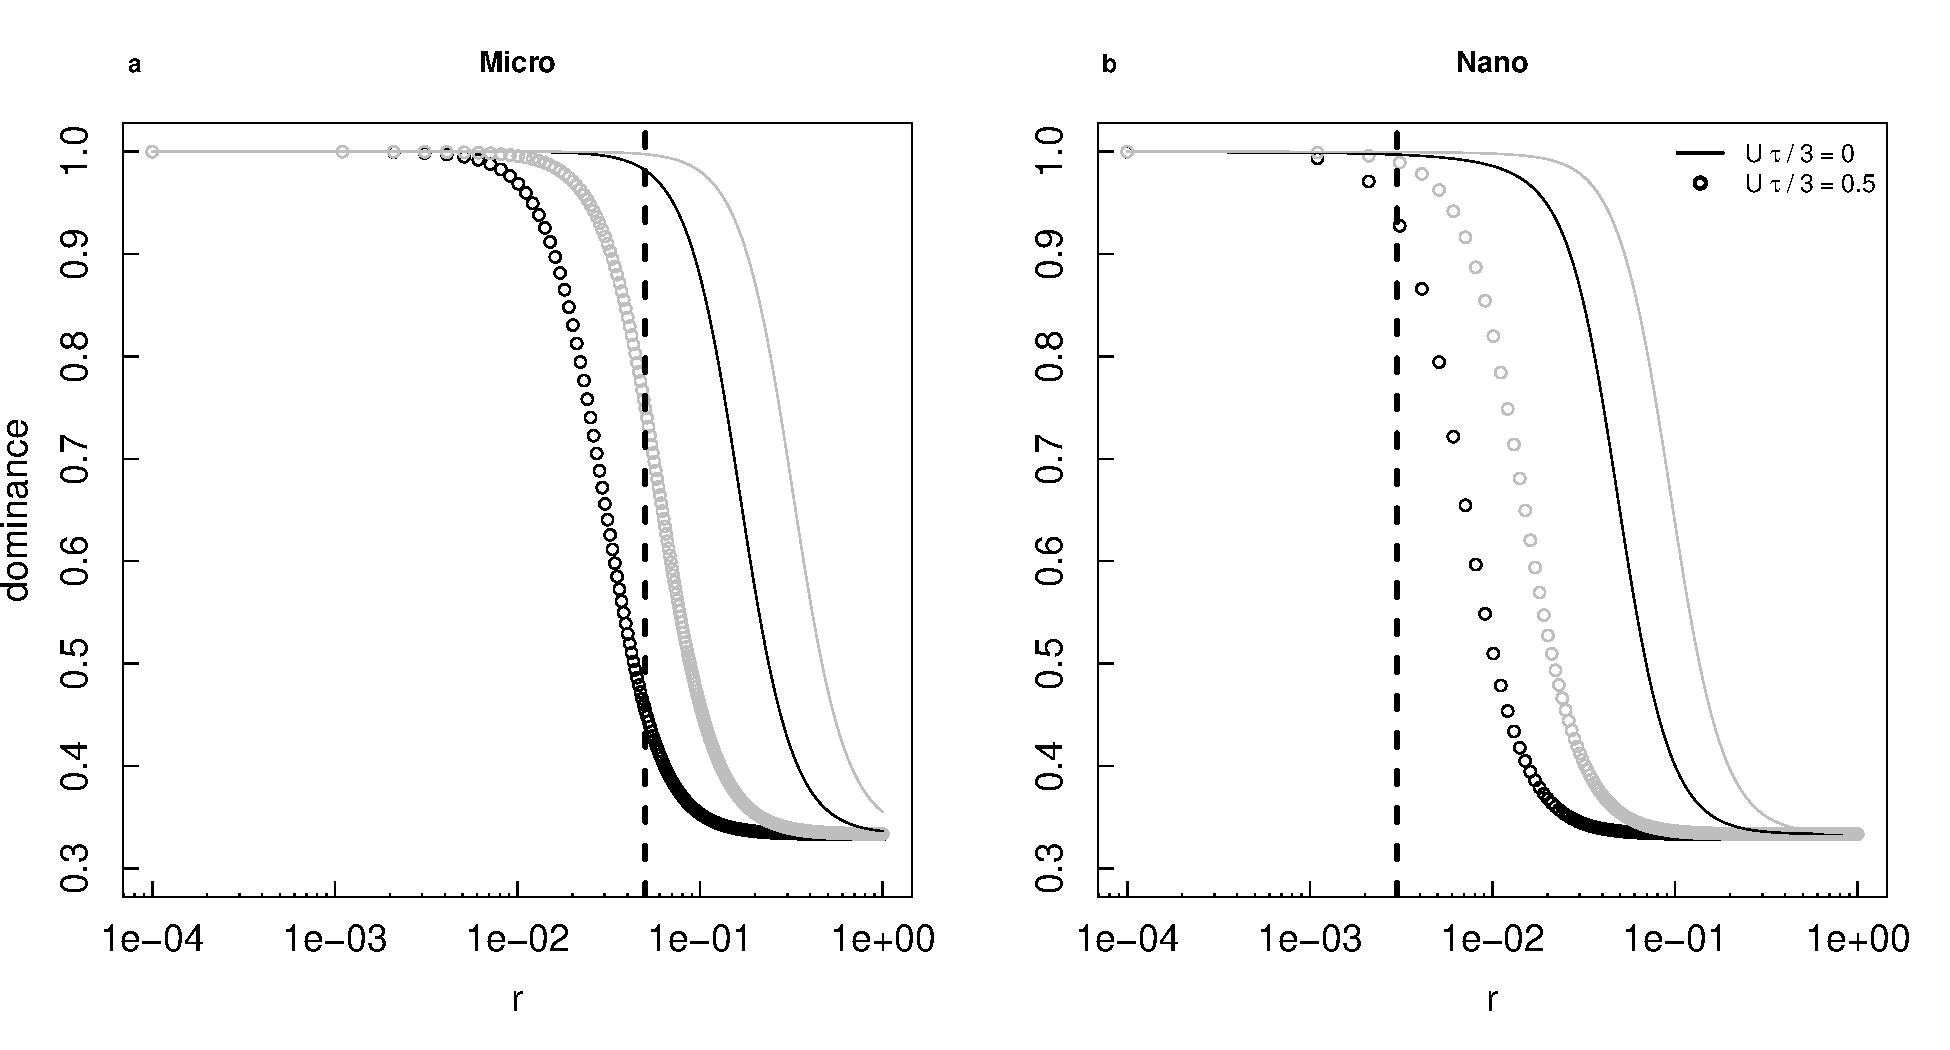
\includegraphics[width=0.99\textwidth]{../code/figure/theoretical_dominance_with_adv} 
\par\end{centering}
\caption{Dominance indices as a function of distance (in cm) for one species
in a microphytoplankton (a) and nanophytoplankton (b) 3-species community
with even distributions after 1000 timesteps with (circles) and without
(lines) advection for different durations of the timesteps, with reference
parameters (black) and lower flow velocity (grey). \label{fig:Dominance_advection}}
\end{figure}

Fig. \ref{fig:Dominance_advection} also functions as a sensitivity analysis of our results with respect to the technical characterization of $U$ (resp. $\gamma$): while decreasing $U$ (resp. $\gamma$) decreases the mixing, so that microphytoplankton could in fact be slightly more aggregated, the dominance index never gets above 0.7 at the interaction radius threshold---the results are not modified substantially. However, combination of such lower $U$ and a slightly lower interaction threshold (see Discussion) may create some intraspecific dominance in microphytoplankton too. 

\section{Minimum distances between individuals}

\subsubsection*{Theory}

One of the reasons why estimating $K(r)$, and even more so $g(r)$,
is difficult is that for small distances (below 10$^{-2}$), we can
find very few observations of pairs of points. In order to better
understand at which distance ranges we should expect some estimation
difficulties, we wanted to compute the minimum expected distance between
points (distance to the nearest neighbour, DNN) when they are uniformly
distributed.

In $d$ dimensions, the probability distribution of the distance $r$
to the nearest-neighbour follows $f(r)=db_{d}Cr^{d-1}\exp(-b_{d}r^{_{d}}C)$
where $C$ is the intensity of the process. If we want to find the
distribution of the minimum DNN between $n$ realized points of a
Poisson process with intensity $C$, we can write 
\begin{equation}
\begin{array}{ccc}
\mathbb{P}(\min(R_{1},...,R_{n})>r) & = & \mathbb{P}(R_{1}>r,...,R_{n}>r)\\
 & = & \Pi_{i=1}^{n}\mathbb{P}(R_{i}>r)\\
 & = & \Pi_{i=1}^{n}\exp(-b_{d}r^{_{d}}C)\\
 & = & \exp(-b_{d}r^{_{d}}\Sigma_{i=1}^{n}C).
\end{array}
\end{equation}

We can then conclude that the distribution of the minimum distance
follows the same distribution as the DNN, but with intensity $nC$.

\medskip{}

\citet{clark_generalization_1979} show that a variable with probability
distribution (with notations changed to fit our own) $f(r)=\frac{dC\pi^{d/2}r^{d-1}}{\Gamma(\frac{d}{2}+1)}\exp(-\frac{C\pi^{d/2}r^{d}}{\Gamma(\frac{d}{2}+1)})=dCb_{d}r^{d-1}\exp(-Cb_{d}r^{d})$
has an expected value of $\mu_{d}=\frac{\left(\Gamma(\frac{d}{2}+1)\right)^{1/d}\Gamma(\frac{1}{d}+1)}{C^{1/d}\pi^{1/2}}$.

With intensity $nC$, we can write $\frac{\left(\Gamma(\frac{d}{2}+1)\right)^{1/d}\Gamma(\frac{1}{d}+1)}{(nC)^{1/d}\pi^{1/2}}$.

\medskip{}

In three dimensions, 
\begin{equation}
\begin{array}{ccc}
\mu_{d} & = & (nC)^{-1/3}\frac{\left(\Gamma(\frac{3}{2}+1)\right)^{1/3}\Gamma(\frac{1}{3}+1)}{\pi^{1/2}}\\
 & = & (nC)^{-1/3}\left(\frac{3}{2}\Gamma(3/2)\right)^{1/3}\frac{1}{3}\Gamma(1/3)\frac{1}{\pi^{1/2}}\\
 & \approx & 0.554\frac{1}{(nC)^{1/3}}.
\end{array}\label{eq:dnn_realization}
\end{equation}

This needs to be taken into account when defining $C$. For microphytoplankton,
using $C=10$ cells~cm$^{-3}$ and $n\approx10^{4}$, the expected
smallest NN distance for a uniform distribution is $1.2\times10^{-2}$
cm. For nanophytoplankton, using $C=10^{3}$ cells~cm$^{-3}$ and
$n\approx10^{4}$, it is reduced to $2.6\times10^{-3}$ cm. \medskip{}


\subsubsection*{Simulations}

We can compute the simulated distance to the nearest neighbour in
the BBM and compare it to what we should obtain with a uniform spatial
distribution: the simulated mean distance to the nearest organism,
regardless of its species, is close to the expected value under a
uniform distribution, but the minimum distance to a conspecific is
much lower than expected (Fig. \ref{fig:Distance_micro} for microphytoplankton,
results are similar for nanophytoplankton).

\begin{figure}[H]
\begin{centering}
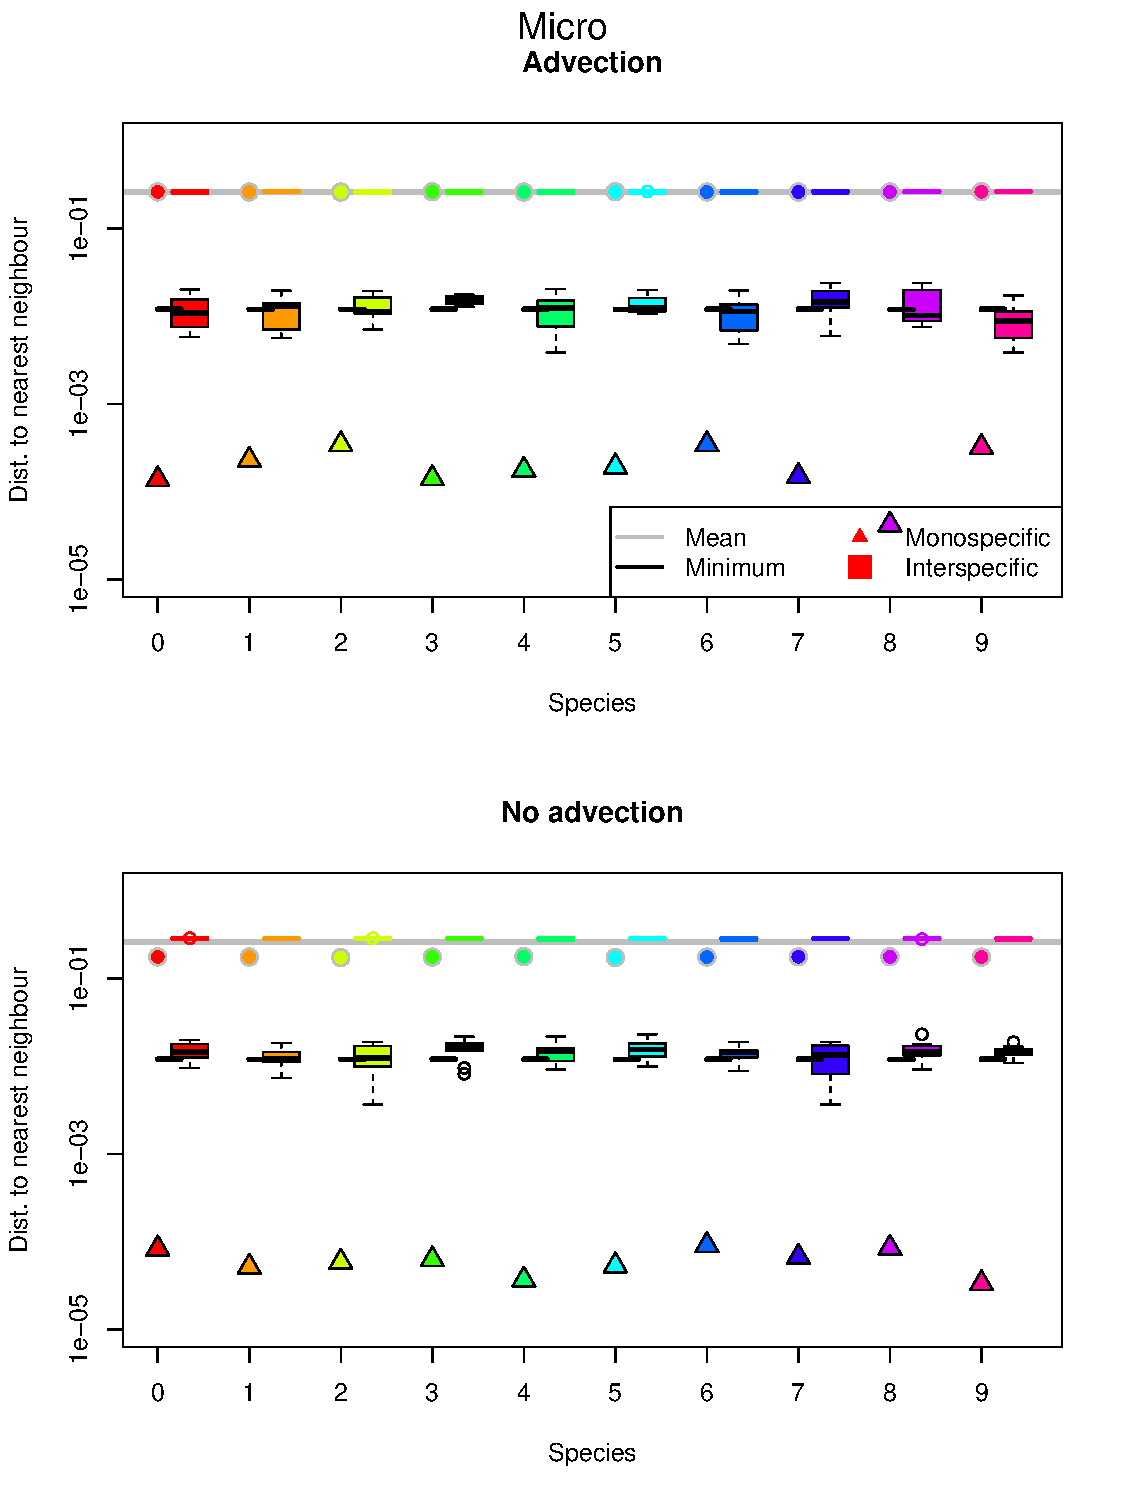
\includegraphics[width=0.85\textwidth]{../code/figure/distrib_distance_micro_box_10sp} 
\par\end{centering}
\caption{Mean and minimum distance (in cm) to the nearest neighbour for 10
microphytoplankton species with density $C=10$ cells~cm$^{-3}$,
with and without advection, after 1000 time steps, compared to predictions
for a uniform distribution. Horizontal lines show the average distance
to the nearest neighbour (grey line) and the expected minimum distance
to the nearest neighbour with the actual number of realizations (black
line). Circles and triangles represent mean and minimum distance to
a conspecific, respectively. Boxplot corresponds to the distribution
of mean (grey outlines) and minimum (black outlines) distances to
a heterospecific. Colors correspond to different species. \label{fig:Distance_micro}}
\end{figure}


\subsubsection*{Relationship with densities}

In the case of a uniform distribution, an increase in density leads
to a decrease in distance to the nearest neighbour (eq. \ref{eq:dnn_realization}).
Mechanically, we can indeed expect that if the number of particles
increases within the same volume, they likely get closer to each other.
We confirm that this is also the case in the Brownian Bug Model.

\begin{figure}[H]
\begin{centering}
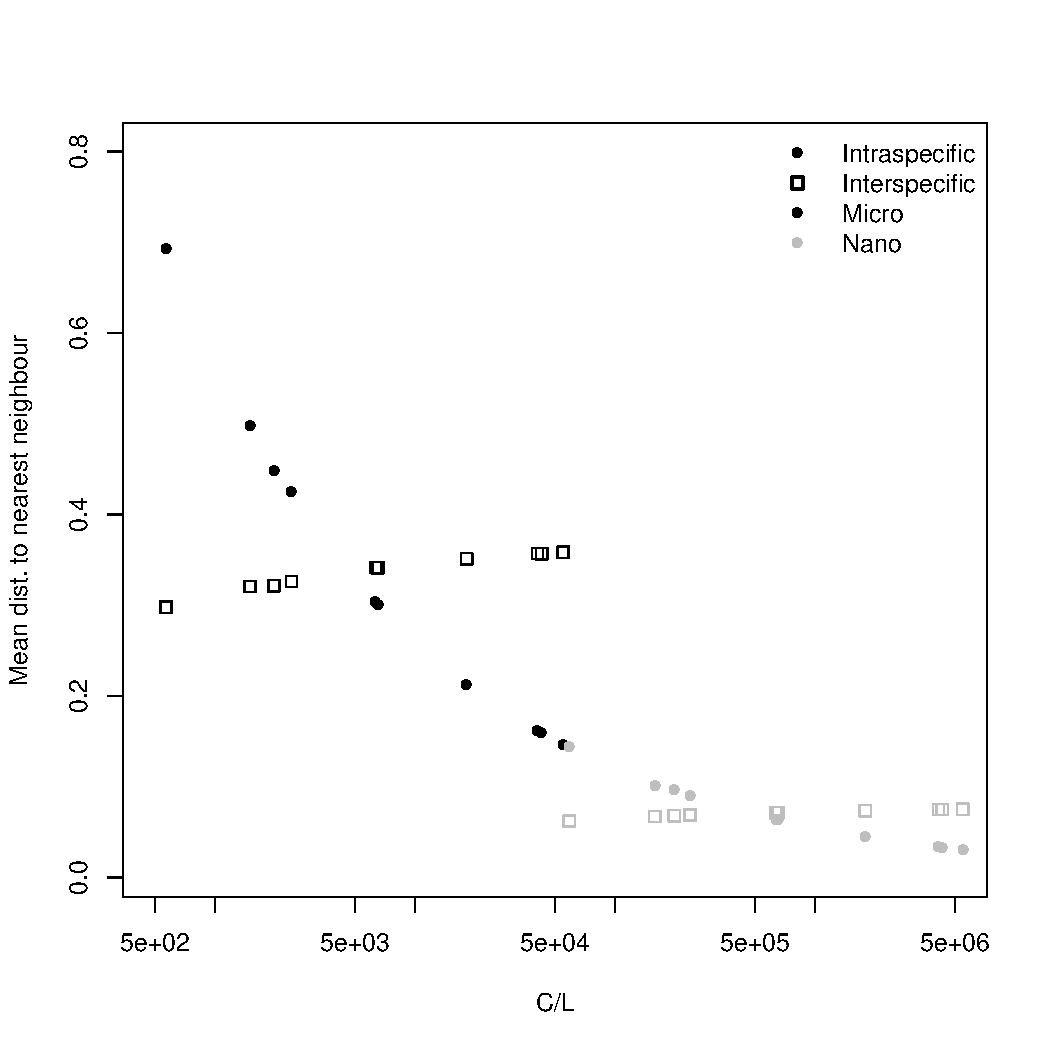
\includegraphics[width=0.75\textwidth]{../code/figure/dist_abundances_10sp_v2} 
\par\end{centering}
\caption{Mean distance (in cm) to the nearest conspecific (filled circle) or
heterospecific (empty square) as a function of density in the environment
for both microphytoplankton (black) and nanophytoplankton (grey) communities
with a skewed abundance distribution, in the presence of advection.\label{fig:Distance_abundance}}
\end{figure}


\section{Relationship between the dominance index, relative strengths of interactions
and coexistence in Lotka-Volterra models}

In this section, we evaluate the potential relationship between local
dominance, ratios of intra-to-interspecific interaction strengths
observed at the population level, and their consequences in a spatial,
dynamic point process Lotka-Volterra framework. Let us define $\mu_{i}$
the average growth rate of a typical individual of species $i$. Assuming
it is linearly dependent on the abundances of the individual's conspecifics
and heterospecifics within a neighbourhood of radius $r$, 
\begin{equation}
\begin{array}{ccc}
\mu_{i}(r,t) & = & b_{i}+\beta_{ii}K_{ii}(r,t)C_{i}(t)+\beta_{io}\Sigma_{j\neq i}K_{ij}(r,t)C_{j}(t)\\
 & = & b_{i}+\beta_{ii}M_{ii}(r,t)+\beta_{io}M_{io}(r,t)
\end{array}\label{eq:lv_individual}
\end{equation}
where $b_{i}$ is the intrinsic individual growth rate, and $\beta_{ii}$/$\beta_{io}$
are individual-level interaction coefficients with a conspecific /
heterospecific, respectively. $C_{j}(t)K_{ij}(r,t)$ is the expected
number of individuals of species $j$ around a typical individual
of species $i$ within a sphere of radius $r$ centered on the focal
individual at time $t$. $M_{ii}(r,t)~=~K_{ii}(r,t)C_{i}(t)$ and
$M_{io}(r,t)~=~\Sigma_{j\neq i}K_{ij}(r,t)C_{j}(t)$.

If we are close to an equilibrium at the local scale, and intra- and
interspecific interaction strengths are equal \textit{at the individual
level} ($\beta_{ii}=\beta_{io}=\beta$), on average, 
\begin{equation}
b_{i}+\beta M_{ii}(r,t)+\beta M_{io}(r,t)\approx0.\label{eq:lv_individual_equilibrium}
\end{equation}

\medskip{}

We can now focus on the dynamics at the community level. We denote
$\alpha_{ij}$ the interactions at population level (by contrast to
$\beta_{ij}$ at individual level, as in \citealp{wiegand_consequences_2021}).
Assuming that all \emph{interspecific} population-level interactions
are similar to one another so that $\alpha_{ij}=\alpha_{io}$ if $j\neq i$,
the per capita growth rate at population level can be written as
\begin{equation}
\begin{array}{ccc}
\frac{1}{C_{i}}\frac{dC_{i}(t)}{dt} & = & b_{i}+\alpha_{ii}C_{i}(t)+\alpha_{io}C_{o}(t)\end{array}\approx0.\label{eq:lv_population}
\end{equation}

We can then write the approximate equalities $\alpha_{ii}\approx\beta\frac{M_{ii}(r,t)}{C_{i}(t)}$
and $\alpha_{io}\approx\beta\frac{M_{io}(r,t)}{C_{o}(t)}$ by matching
Eqs. \ref{eq:lv_individual} and \ref{eq:lv_population}, and obtain
the population-level interaction strength ratio 
\begin{equation}
\begin{array}{ccc}
\frac{\alpha_{io}}{\alpha_{ii}} & \approx & \frac{M_{io}(r,t)}{M_{ii}(r,t)}\frac{C_{i}(t)}{C_{o}(t)}.\end{array}
\end{equation}

Using the formula for the dominance index 
\begin{equation}
\begin{array}{ccc}
\mathcal{D}_{i}(r,t) & = & \frac{M_{ii}(r,t)}{M_{ii}(r,t)+M_{io}(r,t)}\\
\Leftrightarrow\frac{M_{io}(r,t)}{M_{ii}(r,t)} & = & \frac{\left(1-\mathcal{D}_{i}(r,t)\right)}{\mathcal{D}_{i}(r,t)}.
\end{array}\label{eq:dominance}
\end{equation}
Thus the population-level interaction strength ratio can be written
out as a function of the dominance index and of the ratio of conspecific
to heterospecific density: 
\begin{equation}
\frac{\alpha_{io}}{\alpha_{ii}}\approx\frac{\left(1-\mathcal{D}_{i}(r,t)\right)}{\mathcal{D}_{i}(r,t)}\frac{C_{i}(t)}{C_{o}(t)}.
\end{equation}

Let us first focus on microphytoplankton in a 3-species community
with an even distribution of abundances. We know that $\mathcal{D}(d_{\text{threshold}})\approx0.4$
at equilibrium. In this case, $\frac{\left(1-\mathcal{D}_{i}(r,t)\right)}{\mathcal{D}_{i}(r,t)}\frac{C_{i}(t)}{C_{o}(t)}=0.75$.
For nanophytoplankton, $\mathcal{D}(d_{\text{threshold}})\approx0.9$,
thus $\frac{\alpha_{io}}{\alpha_{ii}}\approx0.06$. Both ratios of
population-level interaction strength are below 1, in spite of the
$\beta_{ii}=\beta_{io}=\beta$ assumption, and therefore meet a necessary
condition for diversity maintenance in a Lotka-Volterra model. Similar
calculations for the 10-species communities, combining small dominance
indices to low average concentrations, lead to $\frac{\alpha_{io}}{\alpha_{ii}}\ll1$,
compatible with coexistence \citep{barabas_effect_2016}.

\small
\bibliographystyle{ecol_let}
\bibliography{bibliography}

\end{document}
